\documentclass[UTF8,14pt]{article}
\usepackage[UTF8]{ctex}
\usepackage[a4paper, margin=0.8in,top = 20mm,bottom = 20mm]{geometry}
\usepackage{fancyhdr}
\usepackage{wrapfig}
\usepackage{subfig,graphicx} % Required to insert images
\usepackage{enumitem}
\usepackage{multicol}

% \numberwithin{figure}{subsubsection}
% \numberwithin{table}{subsubsection}
\pagestyle{fancy}
\lhead{天津英赛迪科技有限公司}
\chead{基于树莓派的步进电机图形化程序控制}
\rhead{谢远峰}
\renewcommand\headrulewidth{0.2pt}
\renewcommand\footrulewidth{0.2pt}
\newcommand\sectionone[1]{\centerline{\Large{\bfseries{#1}}}}
\newcommand\sectiontwo[1]{\centerline{\large{\bfseries{#1}}}}
\setlength{\headsep}{4mm}
\setlength{\footskip}{5mm}


\setenumerate[1]{itemsep=0pt,partopsep=0pt,parsep=\parskip,topsep=0pt}
\setitemize[1]{itemsep=0pt,partopsep=0pt,parsep=\parskip,topsep=0pt}
\setdescription{itemsep=0pt,partopsep=0pt,parsep=\parskip,topsep=0pt}
\Huge
\title{基于树莓派的步进电机图形化程序控制}
\begin{document}

\begin{titlepage}
	\begin{center}
		\begin{figure}
			\centering
			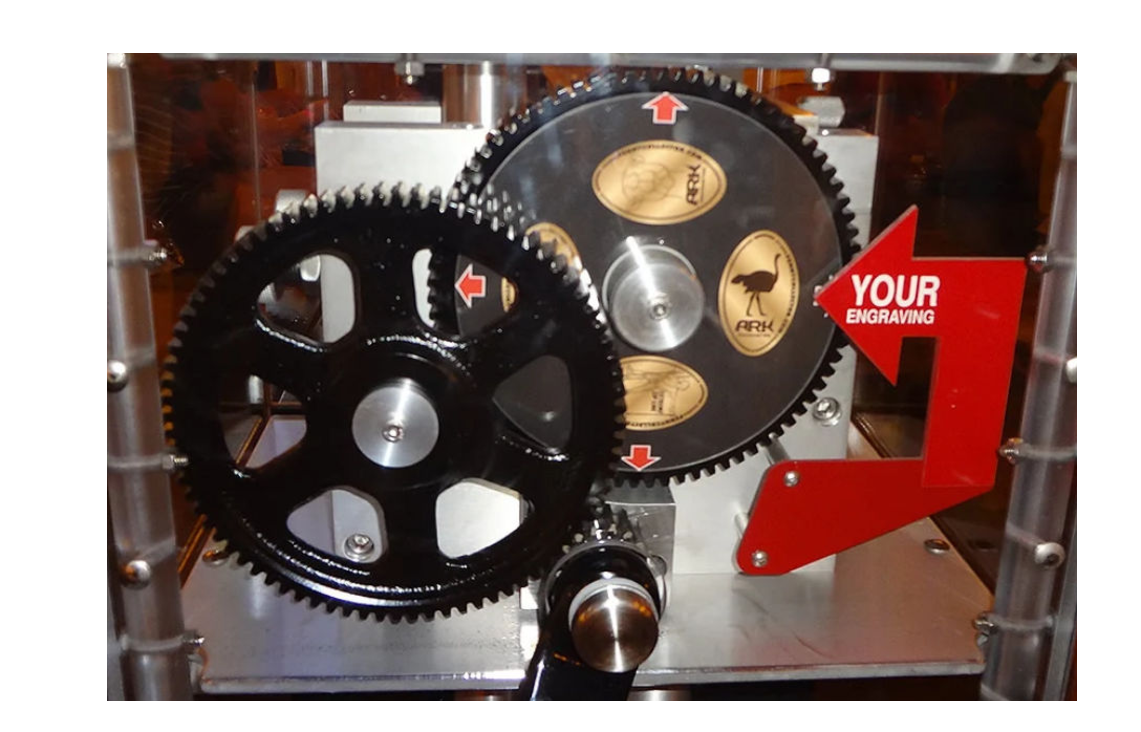
\includegraphics[width=8.2cm]{figures/压币机.pdf}
		\end{figure}
		\vspace{0.2cm}
		\begin{figure}
			\centering
			
\includegraphics[width=4.35cm]{figures/RPi-Logo-Reg-SCREEN.pdf}
		\end{figure}
		\vspace*{0.7cm}
		\line(1,0){300}\\
		[-0.2cm]
		\Huge{\bfseries 压币机自动程序控制}\\
		\vspace*{-0.7cm}
		\line(1,0){300}\\
		\LARGE {基于树莓派的步进电机图形化程序控制\\
			2021年7月22日}\\
		[0.6cm]
		\Large{
			\begin{tabular}{rl}
				单位:         & 天津英赛迪科技有限公司      \\
				姓名        : & 谢远峰                      \\
				时间       :  & 2021年7月22日——2021年8月6日
			\end{tabular}
		}
	\end{center}

\end{titlepage}
\clearpage
\sectionone{摘要}

压币机(自制纪念币)利用机械挤压的方式将硬币进行二次加工,形成一个细长硬币。
新硬币相对于传统硬币被压平或拉伸,并拥有新的设计压花。此类硬币常被用作
纪念或纪念品,在博物馆、游乐园、自然或人造地标等旅游枢纽中常见到压币机。

现代细长硬币是通过将标准的小面额硬币插入小型轧机中制成的,该轧机由两个
相互挤压的钢辊组成,有足够的力使硬币变形。其中一个滚轮(称为“模具”)上
刻有一种设计,当硬币穿过金属时,该设计会在金属上印上新的图像。由此产生的
硬币是椭圆形的,并显示出与磨机模具上的设计相对应的设计。有些机器是手动操
作的,而另一些则是全自动的。

本项目基于树莓派平台,通过外接的可触摸屏幕,利用预先书写的程序,进行印花图案的选择,
通过程序后台与电机控制板的串口通信,调动驱动板控制电机的转动,实现压币机器的自动化
操作。

\vspace{0.5cm}
\sectionone{系统控制需求描述}

\begin{enumerate}
	\item 基于树莓派平台+可触摸屏幕(基于Python-tkinter库的图形化可执行界面程序)
	\item 进入程序主界面,设置连接选项,确保机器与程序能够正常通信(通信异常爆出警告)
	\item 印花图案的选择(程序主页:显示四个图案,代表四种印花格式)
	\item 点选其中一个印花图案,跳出硬币个数界面(暂支持一个),等待用户进行输入
	\item 用户输入后,点击确认,程序发送驱动指令至控制板
	\item 程序向用户发送提示:程序正在运行,等待纪念币的生成(期间页面锁定,不可进行操作)
	\item 指令驱动控制板控制电机进行初始状态的调整(利用旋转编码器获取旋转位置)
	\item 初始状态就位后,发送就绪指令到程序,程序接收后,控制硬币的下落,并驱动电机继续运转
	\item 等待硬币通过滚筒(旋转编码器旋转90-100度)
	\item 发送转动成功消息至程序,程序后端接收后发送至前端,提醒用户纪念币已制成,可拿取
	\item 用户接收到消息,点击消息确认按钮,前端自动返回主页面
\end{enumerate}

\vspace{0.5cm}
\sectionone{功能性需求}
\begin{enumerate}
	\item 能够登录可执行程序主界面
	\item 程序能够为用户提供交互提示性页面(欢迎使用应用,设备已经成功连接)
	\item 程序能够和电机控制板进行串口通信
	\item 程序能够和编码器进行串口通信
	\item 编码器能够获取到电机的转速数据
	\item 编码器通过设置PWM驱动电机的使用
\end{enumerate}

\begin{figure}[h]
	\centering
	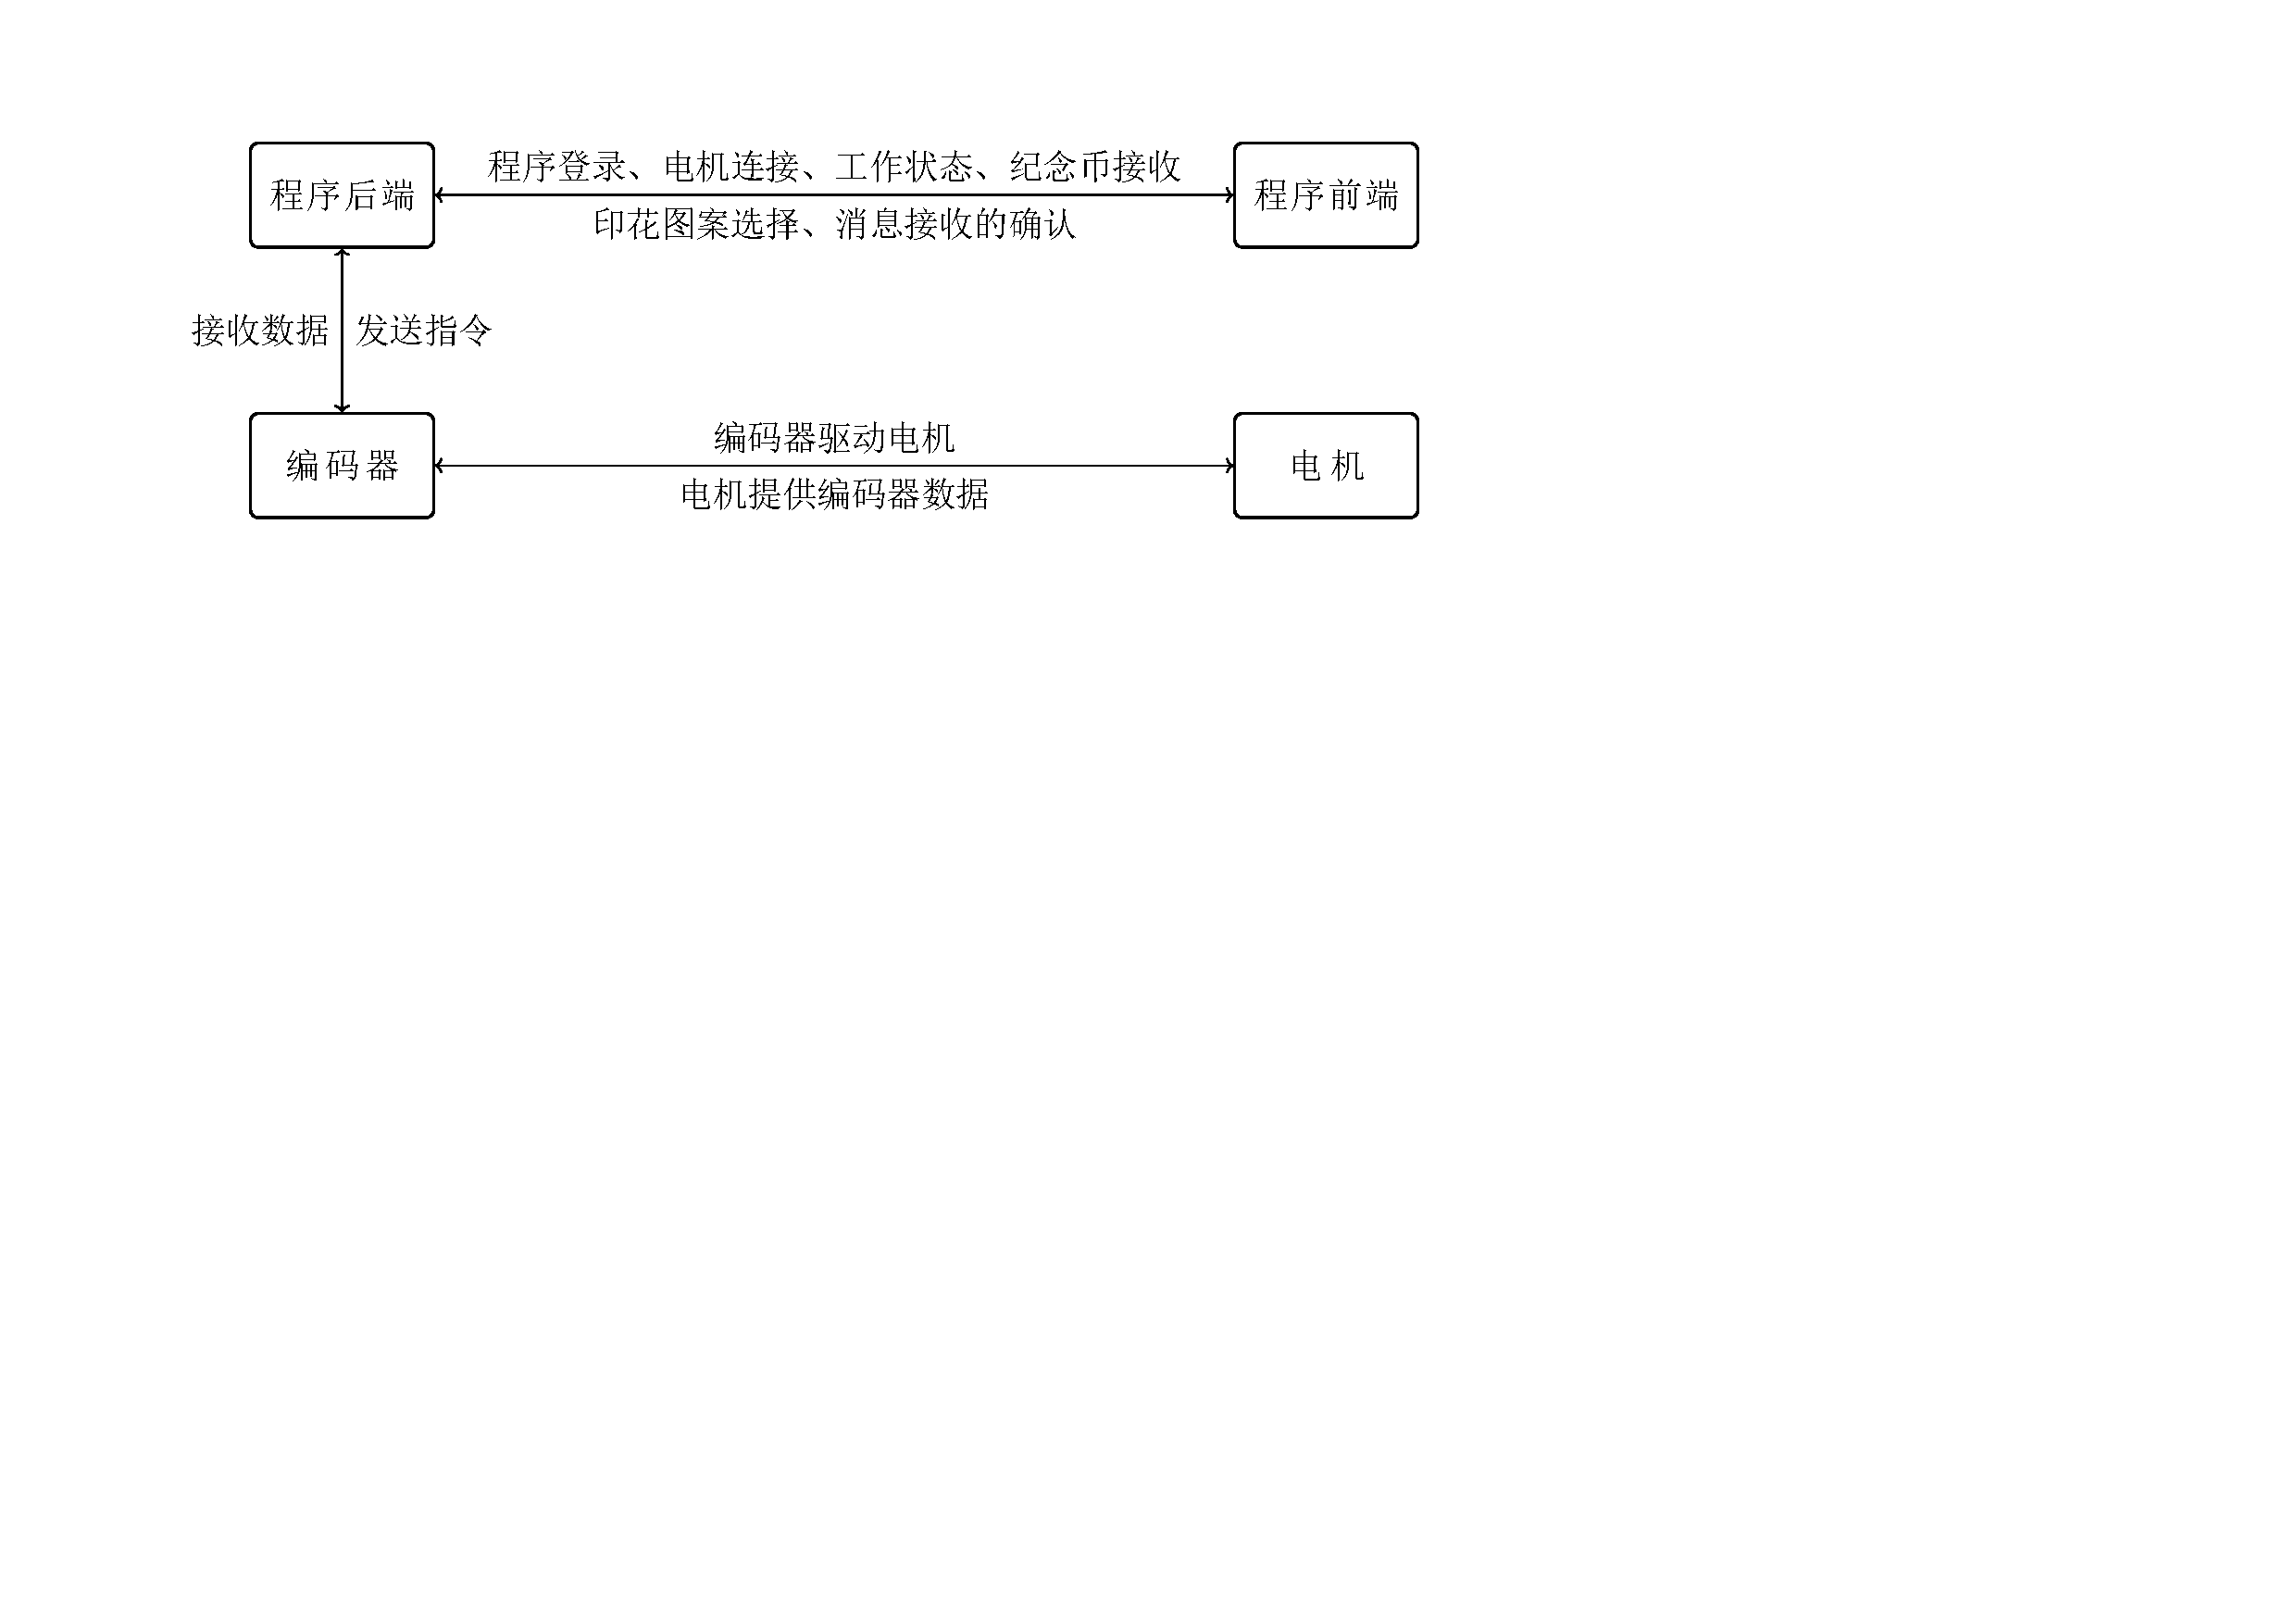
\includegraphics[width=13.5cm]{figures/modlingfig.pdf}
	\vspace{-0.2cm}
	\caption{核心控制流程图}
\end{figure}

\vspace{-0.5cm}
将程序架构分为4个部分:程序前端、程序后端、编码器、电机,程序基于python内置的
tkinter库进行GUI显示,包含程序主界面窗口、登录窗口,压币工作状态窗口、
压币完成窗口。程序内置印花图案点击后,触发对应驱动指令,通过编码器
控制电机转动到指定初始位置,发送信息至用户,提示初始化完成。用户点击确认后,前端
发送系统工作状态提示,后端发送指令控制硬币掉落,滚轮开始转动。
编码器控制的滚轮在转定到一定的角度后,停止工作,向程序发送停止指令。程序接收后,向前端
发送任务已完成,提醒用户拿去纪念币的指令。用户接收到信息,点击确认,程序自动返回主页面。
程序全部流程结束。

\clearpage
\sectionone{非功能性需求}
\begin{enumerate}
	\item 提供纪念币的尺寸输入,指定硬币的尺寸信息
	\item 提供纪念币的数量输入,同一尺寸的硬币数量
	\item 完善的用户反馈(错误和异常提醒)
\end{enumerate}

\vspace{0.5cm}
\sectionone{流程图展示}
\begin{figure}[h]
	\centering
	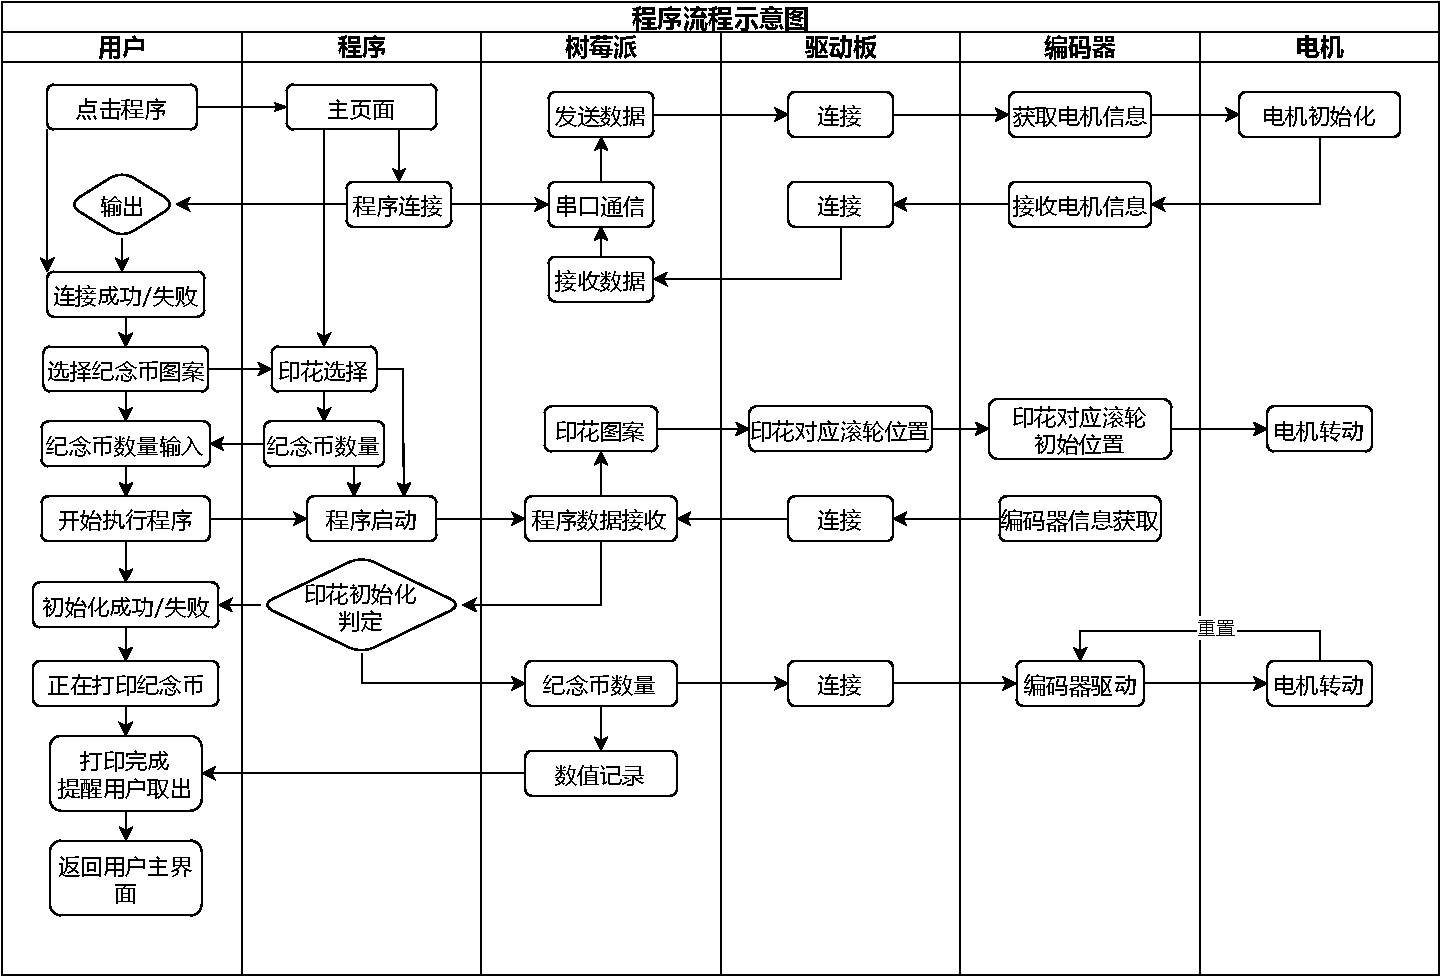
\includegraphics[width=13.5cm]{figures/框架图绘制.pdf}
	\vspace{-10pt}
	\caption{框架图绘制}
	\vspace{-10pt}
\end{figure}

% \vspace{0.5cm}
\sectionone{硬件背景}

\centerline{\large{\bfseries{树莓派4}}}

\begin{wrapfigure}[9]{r}{0.4\textwidth}%靠文字内容的左侧
	\vspace{-0.4cm}
	\centering
	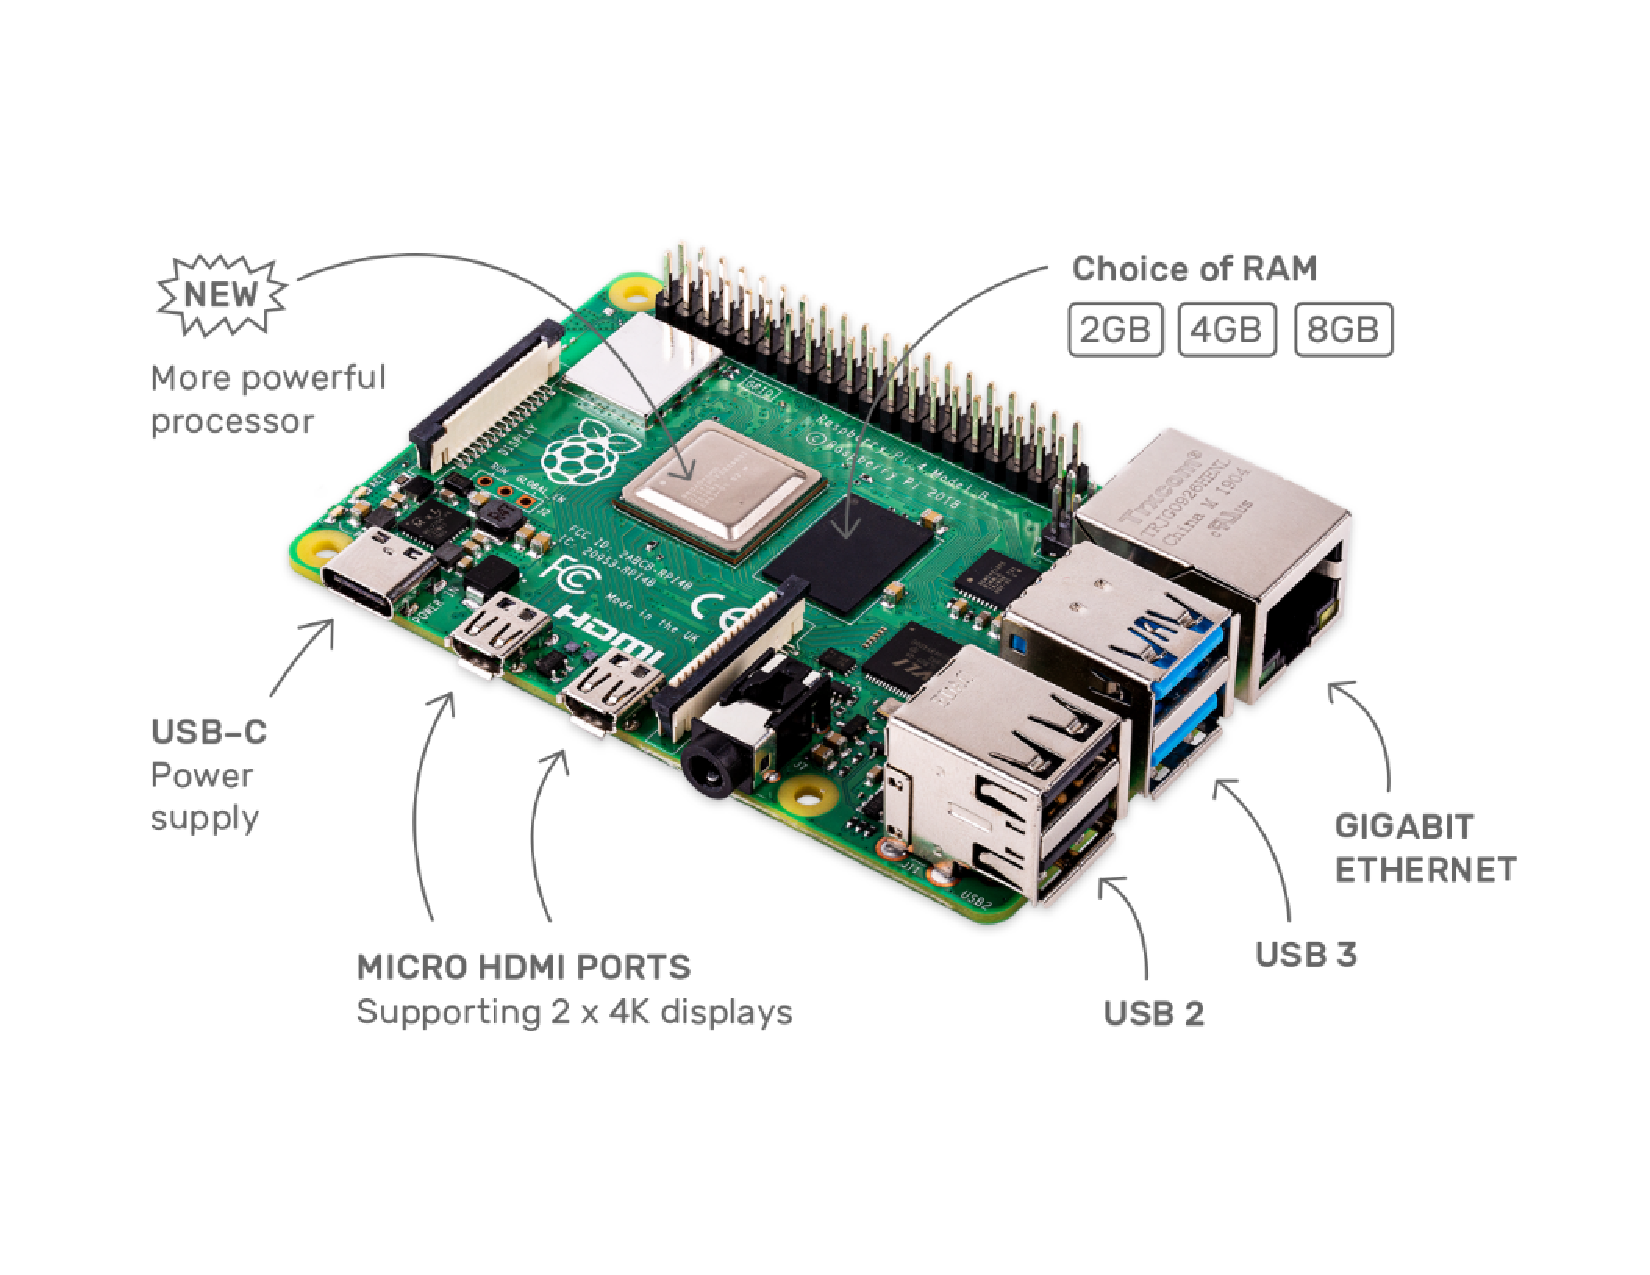
\includegraphics[width=6.75cm]{figures/raspberry4.pdf}
	\vspace{-15pt}
	\caption{树莓派4B接口}
	\vspace{-15pt}
\end{wrapfigure}
树莓派4B是流行的树莓派计算机系列的最新产品,与它的上一代产品树莓派3B+相比,
在处理器速度、丰富的多媒体性能、内存和改进的连接性方面都有显著提高。

树莓派4B拥有64位四核处理器,运行频率为1.5GHz,支持双屏显示,分辨率高达4K、
60fps,最高8GB内存,双频2.4/5.0 GHz无线局域网,蓝牙5.0/BLE,真正的千兆以太网,
USB 3.0,以及PoE功能(通过单独的PoE HAT插件)。

树莓派实质上是一台迷你的嵌入式计算机,利用树莓派可以编辑文档、浏览网页、播放
视频、播放音频等,还可以利用树莓派制作智能小车、电子相框、相机等。

\sectiontwo{可触摸显示屏}
\begin{wrapfigure}[8]{r}{0.35\textwidth}%靠文字内容的左侧
	\vspace{-0.4cm}
	\centering
	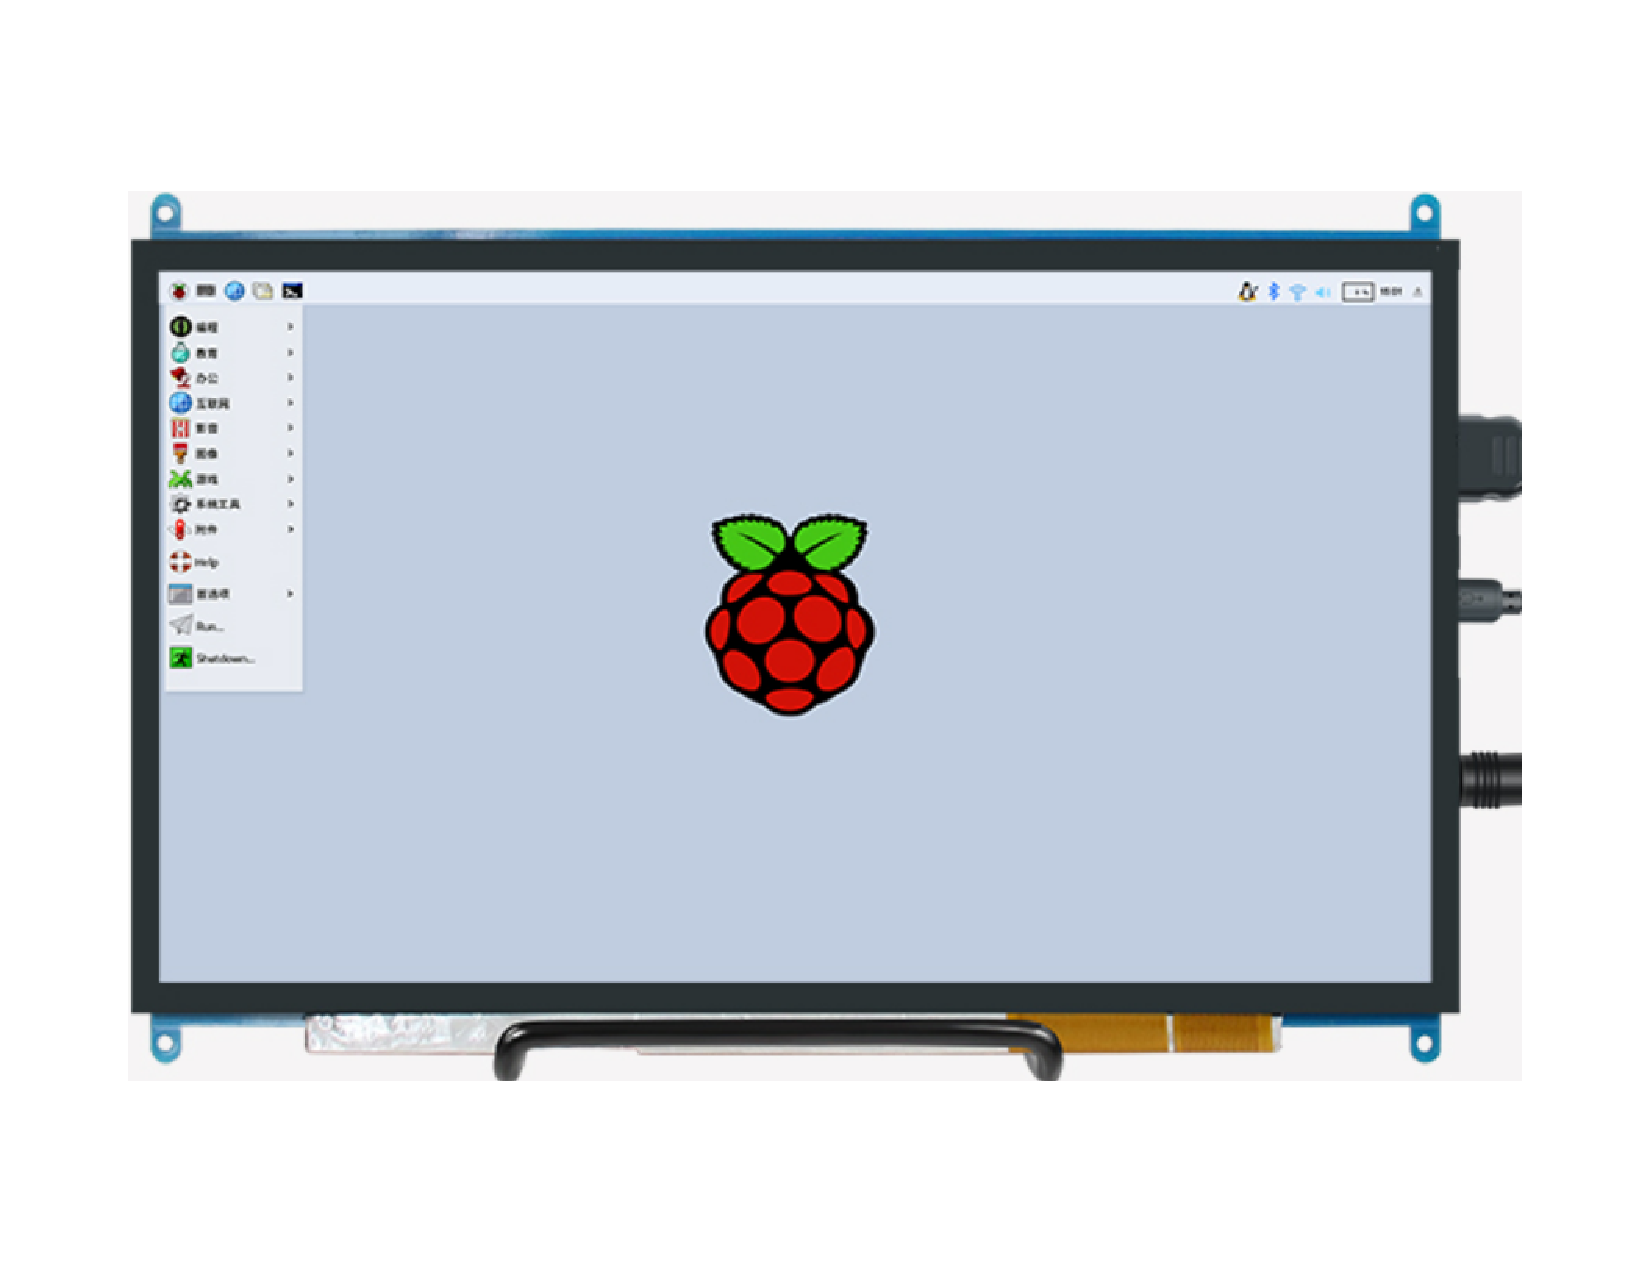
\includegraphics[width=5.56cm]{figures/screen.pdf}
	\vspace{-10pt}
	\caption{可触摸显示屏}
	\vspace{-15pt}
\end{wrapfigure}
创乐博可触摸显示屏,1920x1080分辨率,13.3英寸,支持HD高清显示,可作为
电脑副屏,兼容并可直接插入任何树莓派主板,支持Raspberry系统、Ubuntu系统
、英伟达,十点触控,免驱动安装。USB-12V直流供电。

HDMI接口与树莓派4B主板进行连接,作为程序的GUI界面的直接触控操作板。可直接显示
程序的前端操作页面。USB接口连接USB2.0接口,负责屏幕的触控功能。电路接口支持12V-1A
的适配电源控制。接口成功连接后,启动树莓派系统,等待10秒后,显示Raspberry系统的
主页面,桌面能够正常显示。


\sectiontwo{编码器}
\begin{wrapfigure}[17]{r}{0.35\textwidth}%靠文字内容的左侧
	\vspace{-0.4cm}
	\centering
	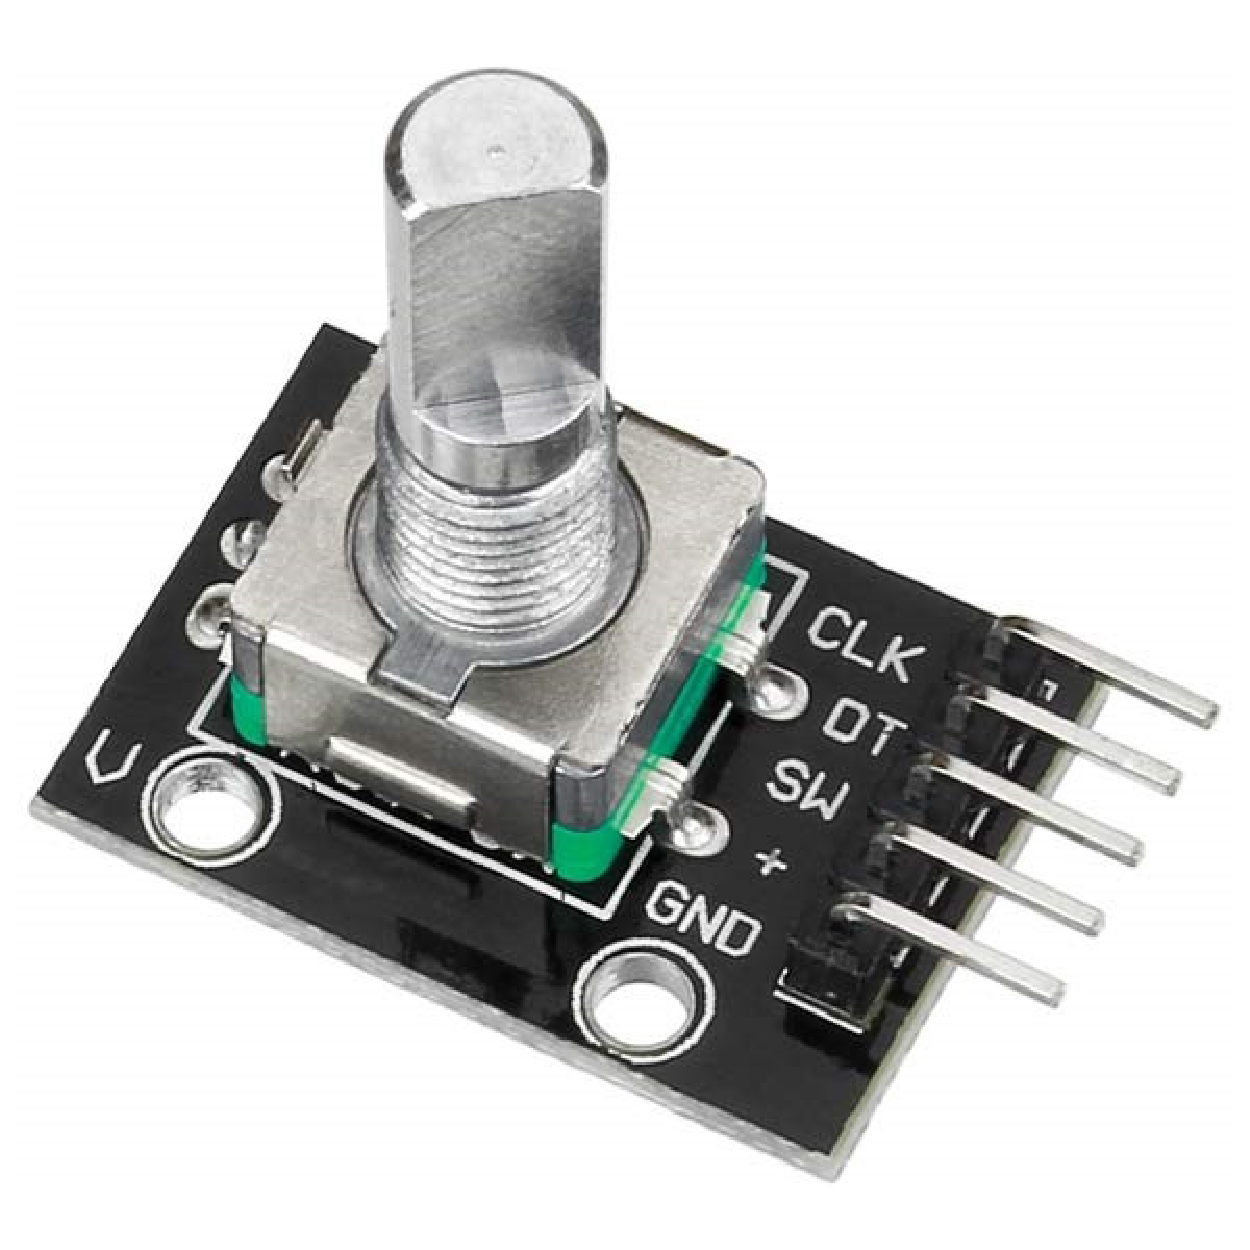
\includegraphics[width=4.89cm]{figures/Ratary_Encoder.pdf}
	\vspace{-10pt}
	\caption{编码器模块}
	% \vspace{-2pt}
	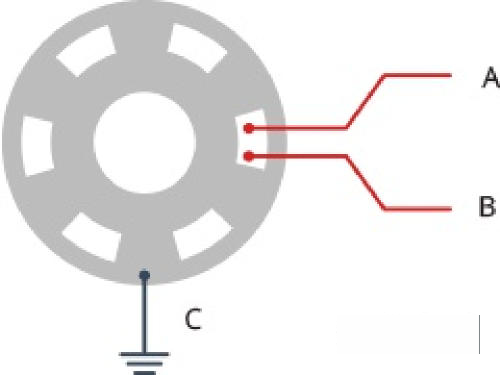
\includegraphics[width=4.25cm]{figures/mapan.pdf}
	\vspace{-5pt}
	\caption{编码盘}
	\vspace{-10pt}
\end{wrapfigure}
旋转编码器是一种位置传感器,可将旋钮的角位置(旋转)转换为用于确定旋钮旋转方向
的输出信号。由于其坚固性和良好的数字控制;它们被用于许多应用中,包括机器人技术,
CNC机器和打印机。

旋转编码器有两种类型-绝对式和增量式。绝对编码器为我们提供旋钮的精确位置(以度为
单位),而增量编码器报告轴已移动了多少增量。相较于电位器,旋转编码器能够提供实时
的位置变化。

\begin{itemize}
	\item \textbf{GND}为接地输出
	\item \textbf{VCC}为正电源电压,通常为3.3或5V
	\item \textbf{SW}为低电平有效的按钮开关输出。按下旋钮时,电压变低。
	\item \textbf{DT(输出B)}与CLK输出相同,可用于确定旋转方向。
	\item \textbf{CLK(输出A)}是确定旋转量的主要输出脉冲。
\end{itemize}

编码器内部是一个槽形磁盘,该磁盘连接到公共接地引脚C以及两个接触针A和B,如图5所示。
旋转旋钮时,A和B根据旋转旋钮的方向以特定顺序与公共接地引脚C接触。当接触公共接地
时,针脚产生信号。一个引脚先于另一引脚接触,信号会有90°的相位差。称为
\textbf{正交编码}。顺时针旋转旋钮时,首先连接A引脚,然后连接B引脚。逆时针旋转旋钮时
,首先连接B引脚,然后连接A引脚。通过跟踪每个引脚何时与地面连接或与地面断开,可以使用
这些信号变化来确定旋钮的旋转方向。通过在A更改状态时观察B的状态来做到这一点。状态相同
时,指示旋钮顺时针转动;状态不同,指示旋钮逆时针转动。

% \clearpage
% \centerline{\large{\bfseries{霍尔编码器电机}}}
\vspace{0.5cm}
\sectiontwo{L298N模块}
\begin{wrapfigure}[12]{r}{0.4\textwidth}%靠文字内容的左侧
	\vspace{-0.4cm}
	\centering
	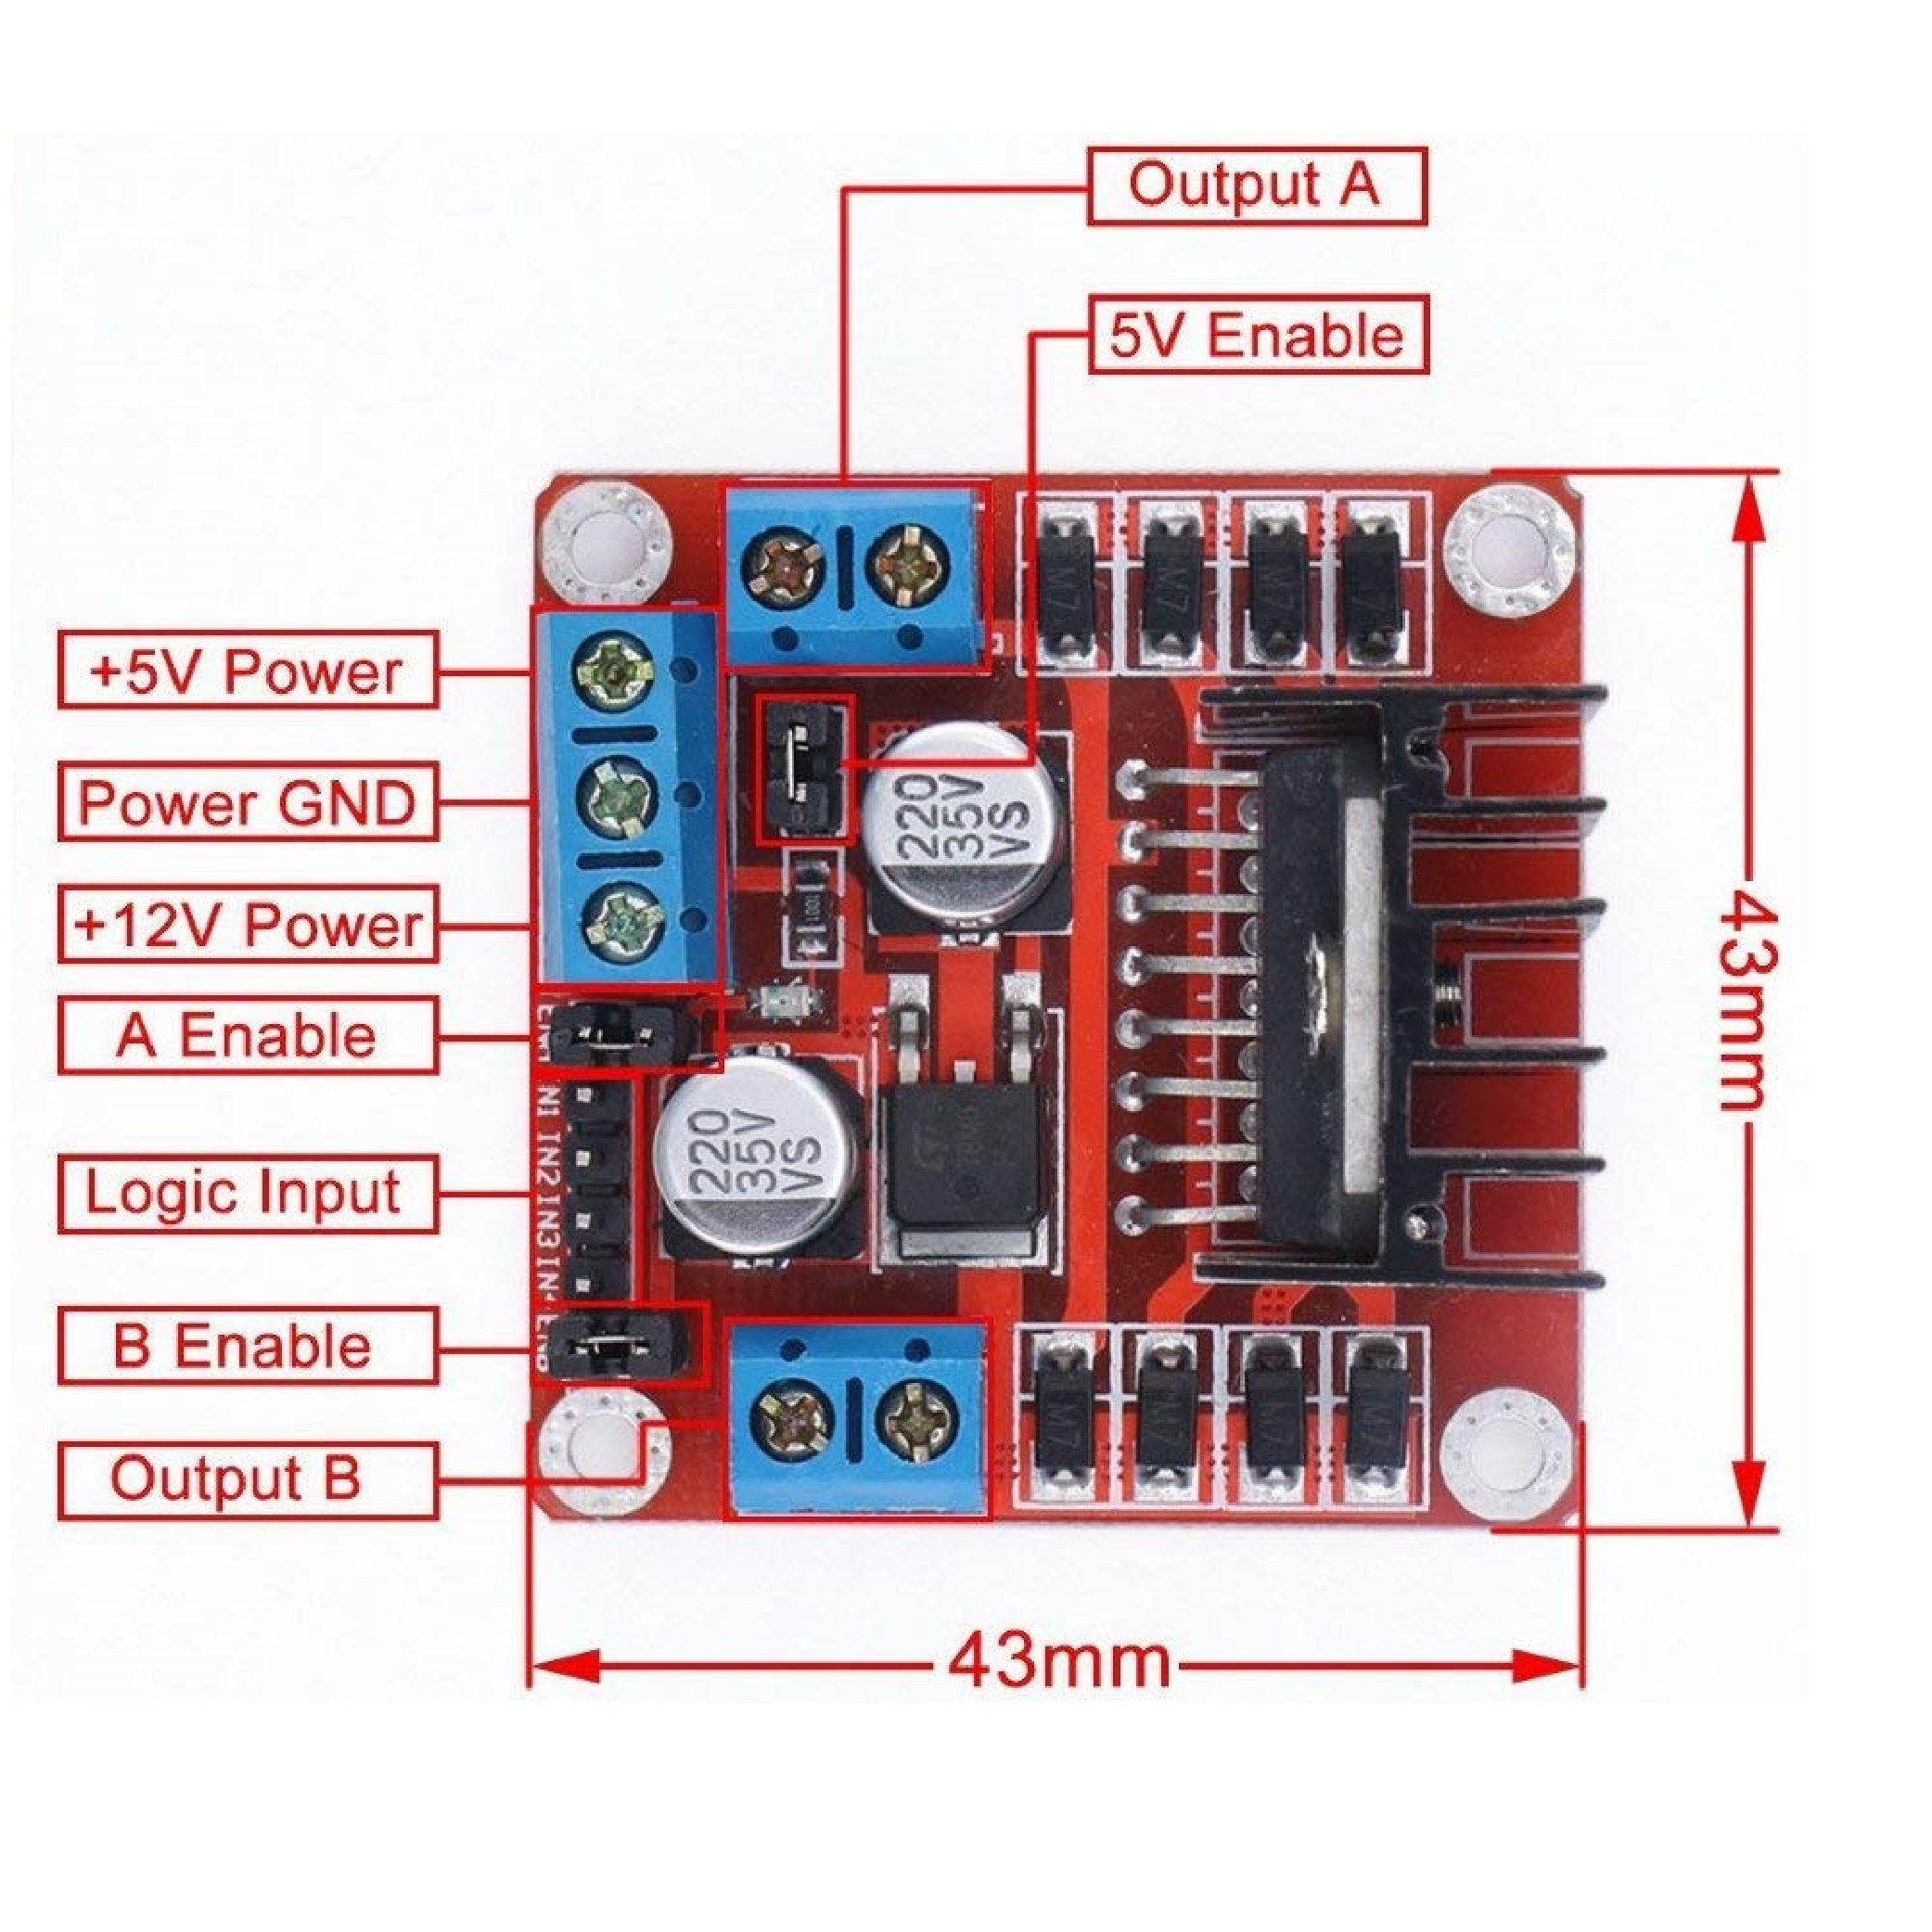
\includegraphics[width=6.56cm]{figures/motor-driver.pdf}
	\vspace{-10pt}
	\caption{L298N电机驱动板接口说明}
	\vspace{-15pt}
\end{wrapfigure}
引脚说明
\begin{enumerate}
	\item \textbf{VCC输入}:L298N芯片的电源正极,范围可以是5V$\sim$35V,如果需从模块内取电给树莓派供电,则其范围为7V$\sim$35V。
	\item \textbf{GND}:L298N芯片的电源地,使用的时候应该把树莓派的GND接到这里,即两者需要共地,否则电机不转。
	\item \textbf{+5V输出}:L298N芯片输出的5V电源,可以给外部设备供电,但要求VCC输入要达到7V以上
	\item \textbf{ENA、ENB}:A、B通道的使能端,高电平有效,向使能端输入不同占空比的PWM脉冲信号可控制电机转速。使用时接到树莓派的GPIO上,实现程序控制。
	\item \textbf{INA、INB、INC、IND}:INA、INB为A通道的控制输入,INC、IND为B通道的控制输入。
	\item \textbf{OUTA、OUTB}为A通道输出,为电机提供电源。
	\item \textbf{OUTC、OUTD}为B通道输出,为电机提供电源。
\end{enumerate}

\vspace{0.3cm}
\sectiontwo{步进电机}
\begin{wrapfigure}[10]{R}{0.21\textwidth}
	\centering
	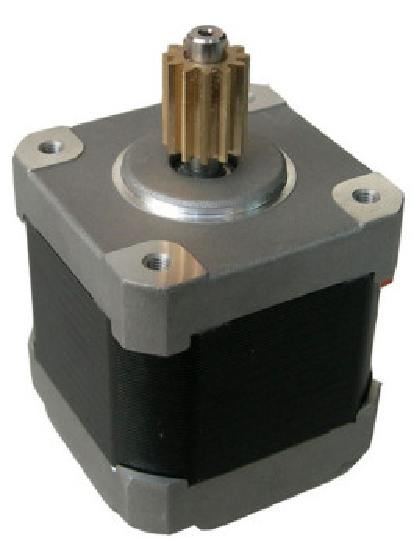
\includegraphics[width=2.5cm]{figures/bujindianji.pdf}
	\vspace{-10pt}
	\caption{步进电机}
	\vspace{-15pt}
\end{wrapfigure}
{\bfseries{步进电机介绍:}}

步进电机是一种将电脉冲信号转换成相应角位移或线位移的电动机。
每输入一个脉冲信号,转子就转动一个角度或前进一步,其输出的
角位移或线位移与输入的脉冲数成正比,转速与脉冲频率成正比。因
此,步进电动机又称脉冲电动机。

1.步进电机是一种无刷直流电机,可将360°的完整旋转角度分成相等的步数。

2.通过施加定量控制信号旋转电动机。改变控制信号速率改变旋转速度。

3.Raspberry Pi的GPIO可生成控制信号,用于控制步进电机的旋转。


\clearpage
% \vspace{0.5cm}
\sectionone{确认事项}
\begin{itemize}
	\item 机械装置的原理图获取
	\item 电机是否自带编码器
	\item 程序完成预期确认
	\item 编码器的购买或重用(增量式编码器和绝对式编码器)
	\item 关于指定步进电机的型号、控制板、驱动板的型号,说明书
	\item 说明文档的完善信息
\end{itemize}

\vspace{0.5cm}
\sectionone{备忘录}
\begin{itemize}
	\item 霍尔编码器是增量编码器下的一个种类
	\item python的GUI编程选用tkinter内置库
	\item 串口通信选用第三方工具
\end{itemize}

\vspace{0.5cm}
\sectionone{项目工作安排}
\begin{itemize}
	\item 阅读提供的说明文档资料
	\item 需求确认
	\item 步进电机 编码器资料整理
	\item 树莓派与主机通信
	\item Arduino与带编码器电机的信息通信实现
	\item 树莓派与带编码器电机的串口通信
\end{itemize}

\sectionone{参考资料}
\begin{enumerate}
	\item 树莓派4B介绍——https://www.raspberrypi.org/products/raspberry-pi-4-model-b/
	\item 可触摸显示屏介绍——https://i-item.jd.com/10027470782200.html\#crumb-wrap
	\item 旋转编码器原理介绍和应用——https://zhuanlan.zhihu.com/p/349824627
	\item 霍尔编码器原理介绍和应用——https://blog.csdn.net/robotixworkshop/article/details/114275629
	\item 编码器计数原理与电机测速原理——https://zhuanlan.zhihu.com/p/350368518
	\item L298N模块驱动直流电机实验——https://www.jianshu.com/p/dc71346a2fdf
	\item Arduino实现霍尔编码减速电机PI调速——http://www.cxyzjd.com/article/C1664510416/107227754
	\item 编码器类型原理介绍——https://blog.csdn.net/QWQ\_DIODA/article/details/116519580
	\item Introduction to L298——https://www.theengineeringprojects.com/2017/07/introduction-to-l298.html
	\item How to use the L298N Motor Driver——https://create.arduino.cc/projecthub/ryanchan/how-to-use-the-l298n-motor-driver-b124c5
\end{enumerate}


\clearpage
\sectionone{附录}
\sectiontwo{针脚说明图}
\begin{figure}[!h]
	\centering
	\vspace{-10pt}
	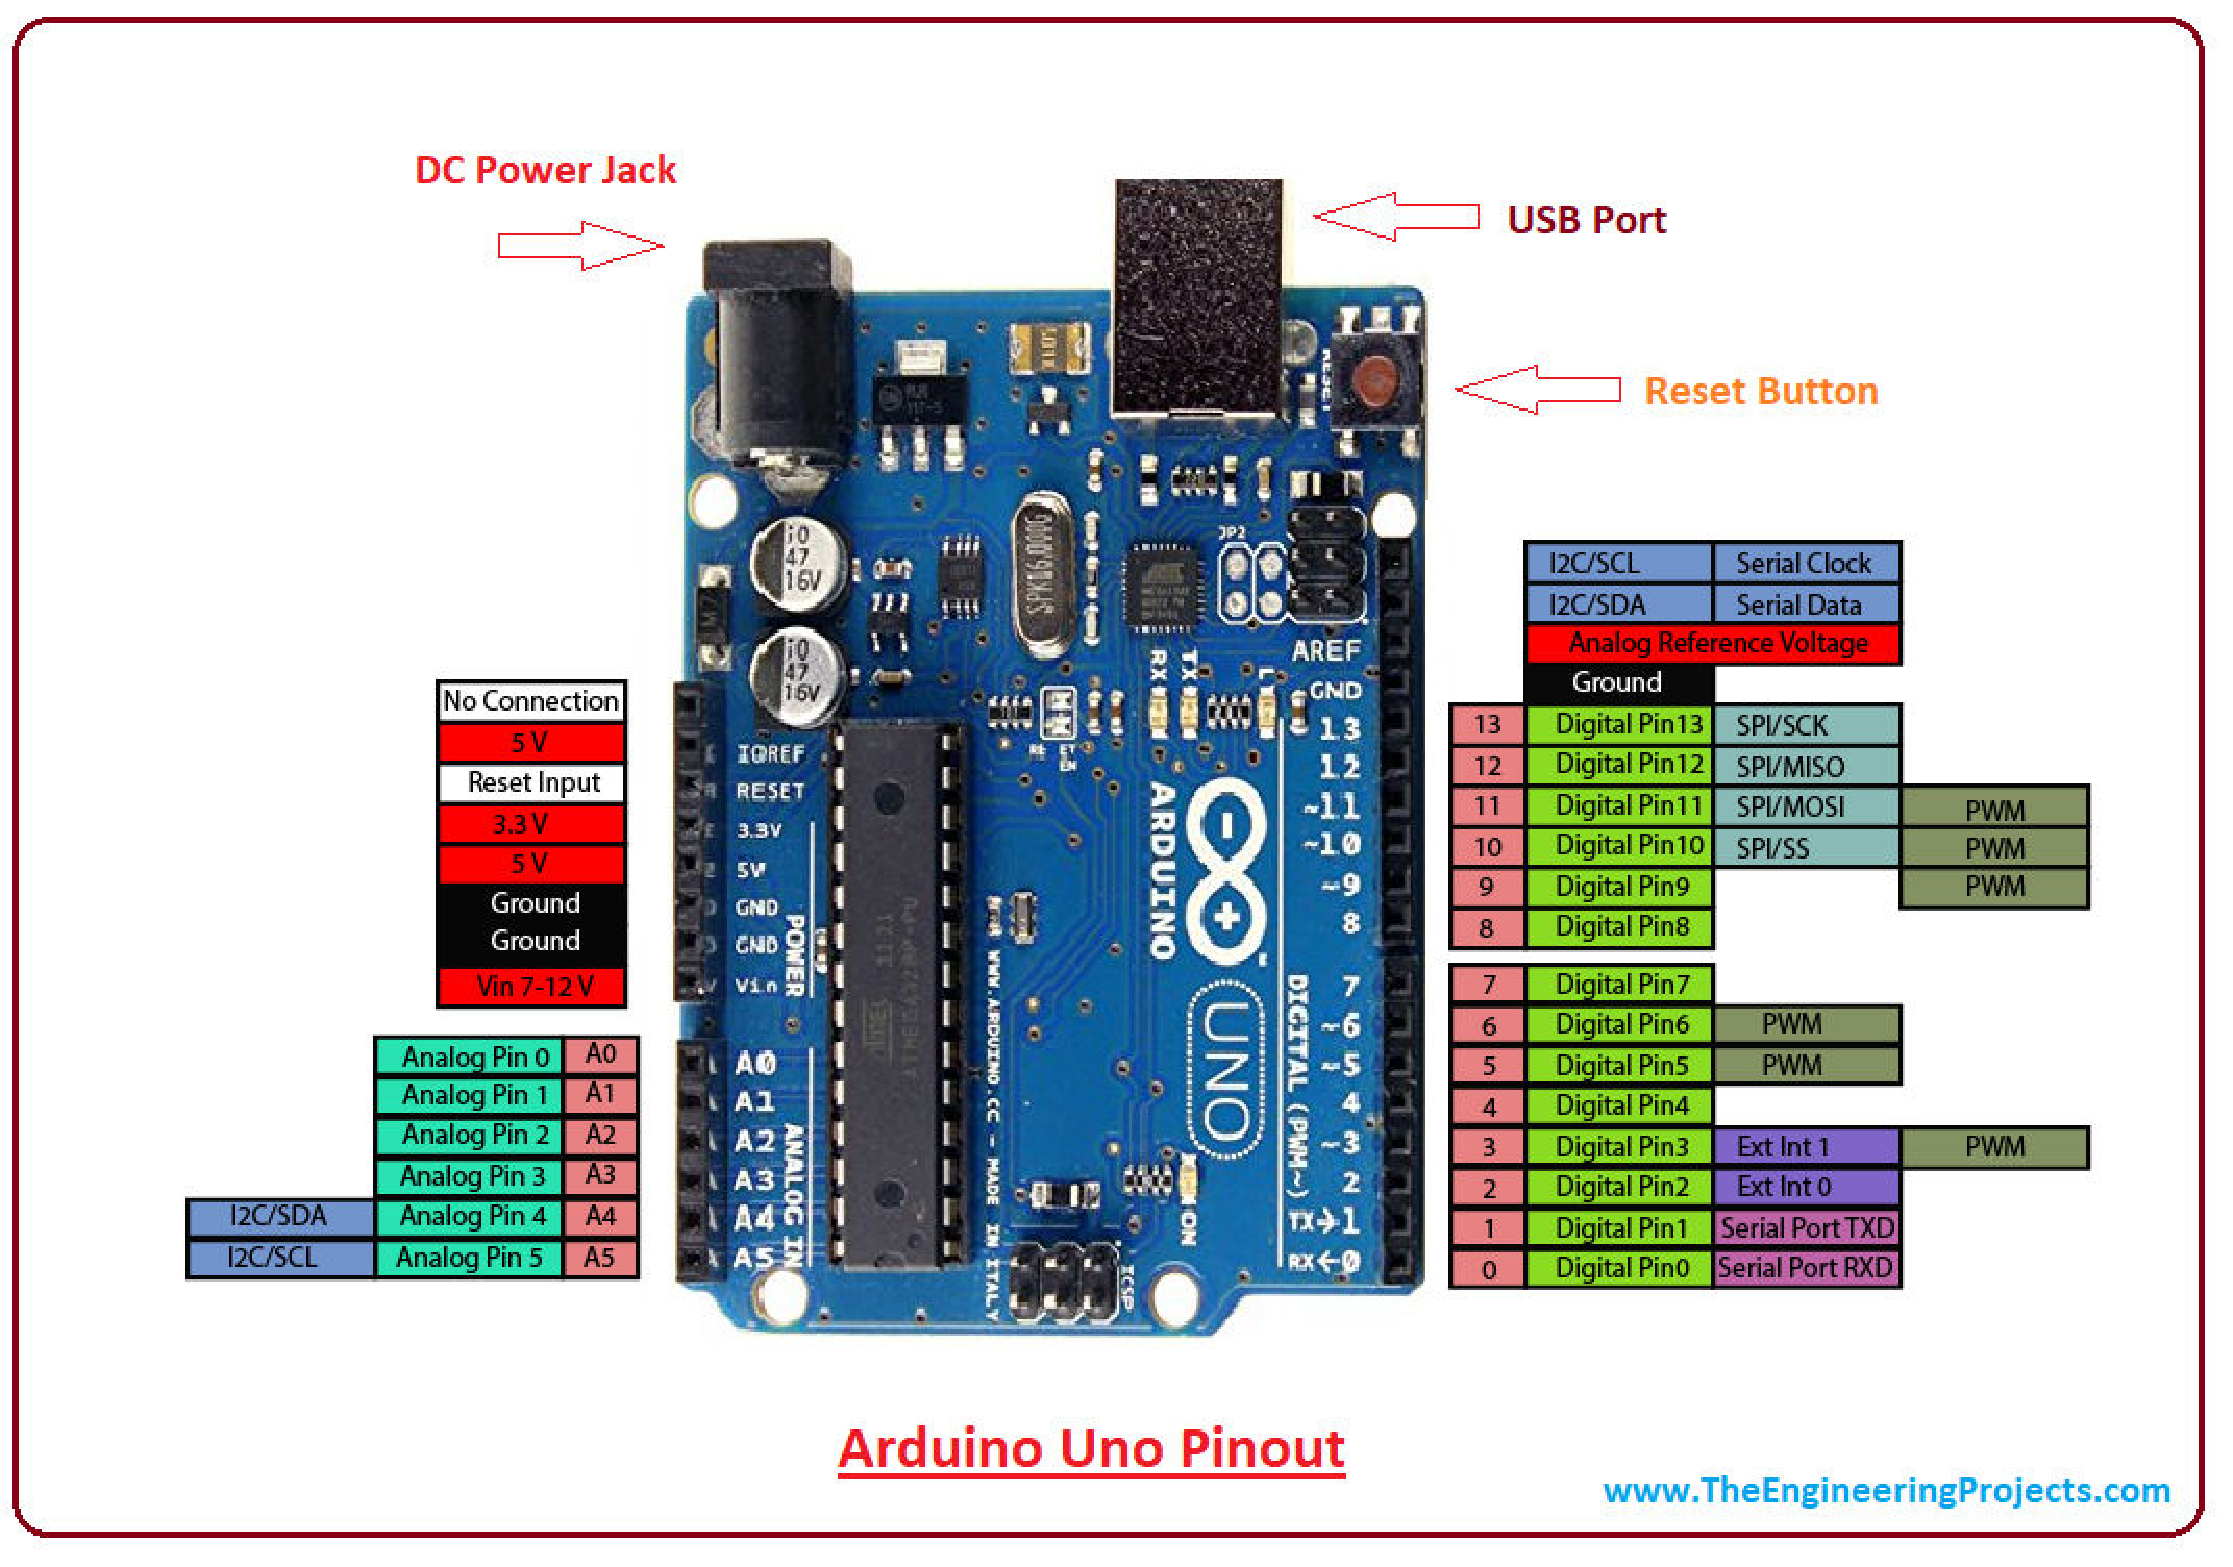
\includegraphics[width=14cm]{figures/arduino-uno.pdf}
	% \vspace{-15pt}
	\caption{Arduino针脚}
	\vspace{-15pt}
\end{figure}

\vspace{1cm}
\begin{figure}[!h]
	\centering
	\vspace{-10pt}
	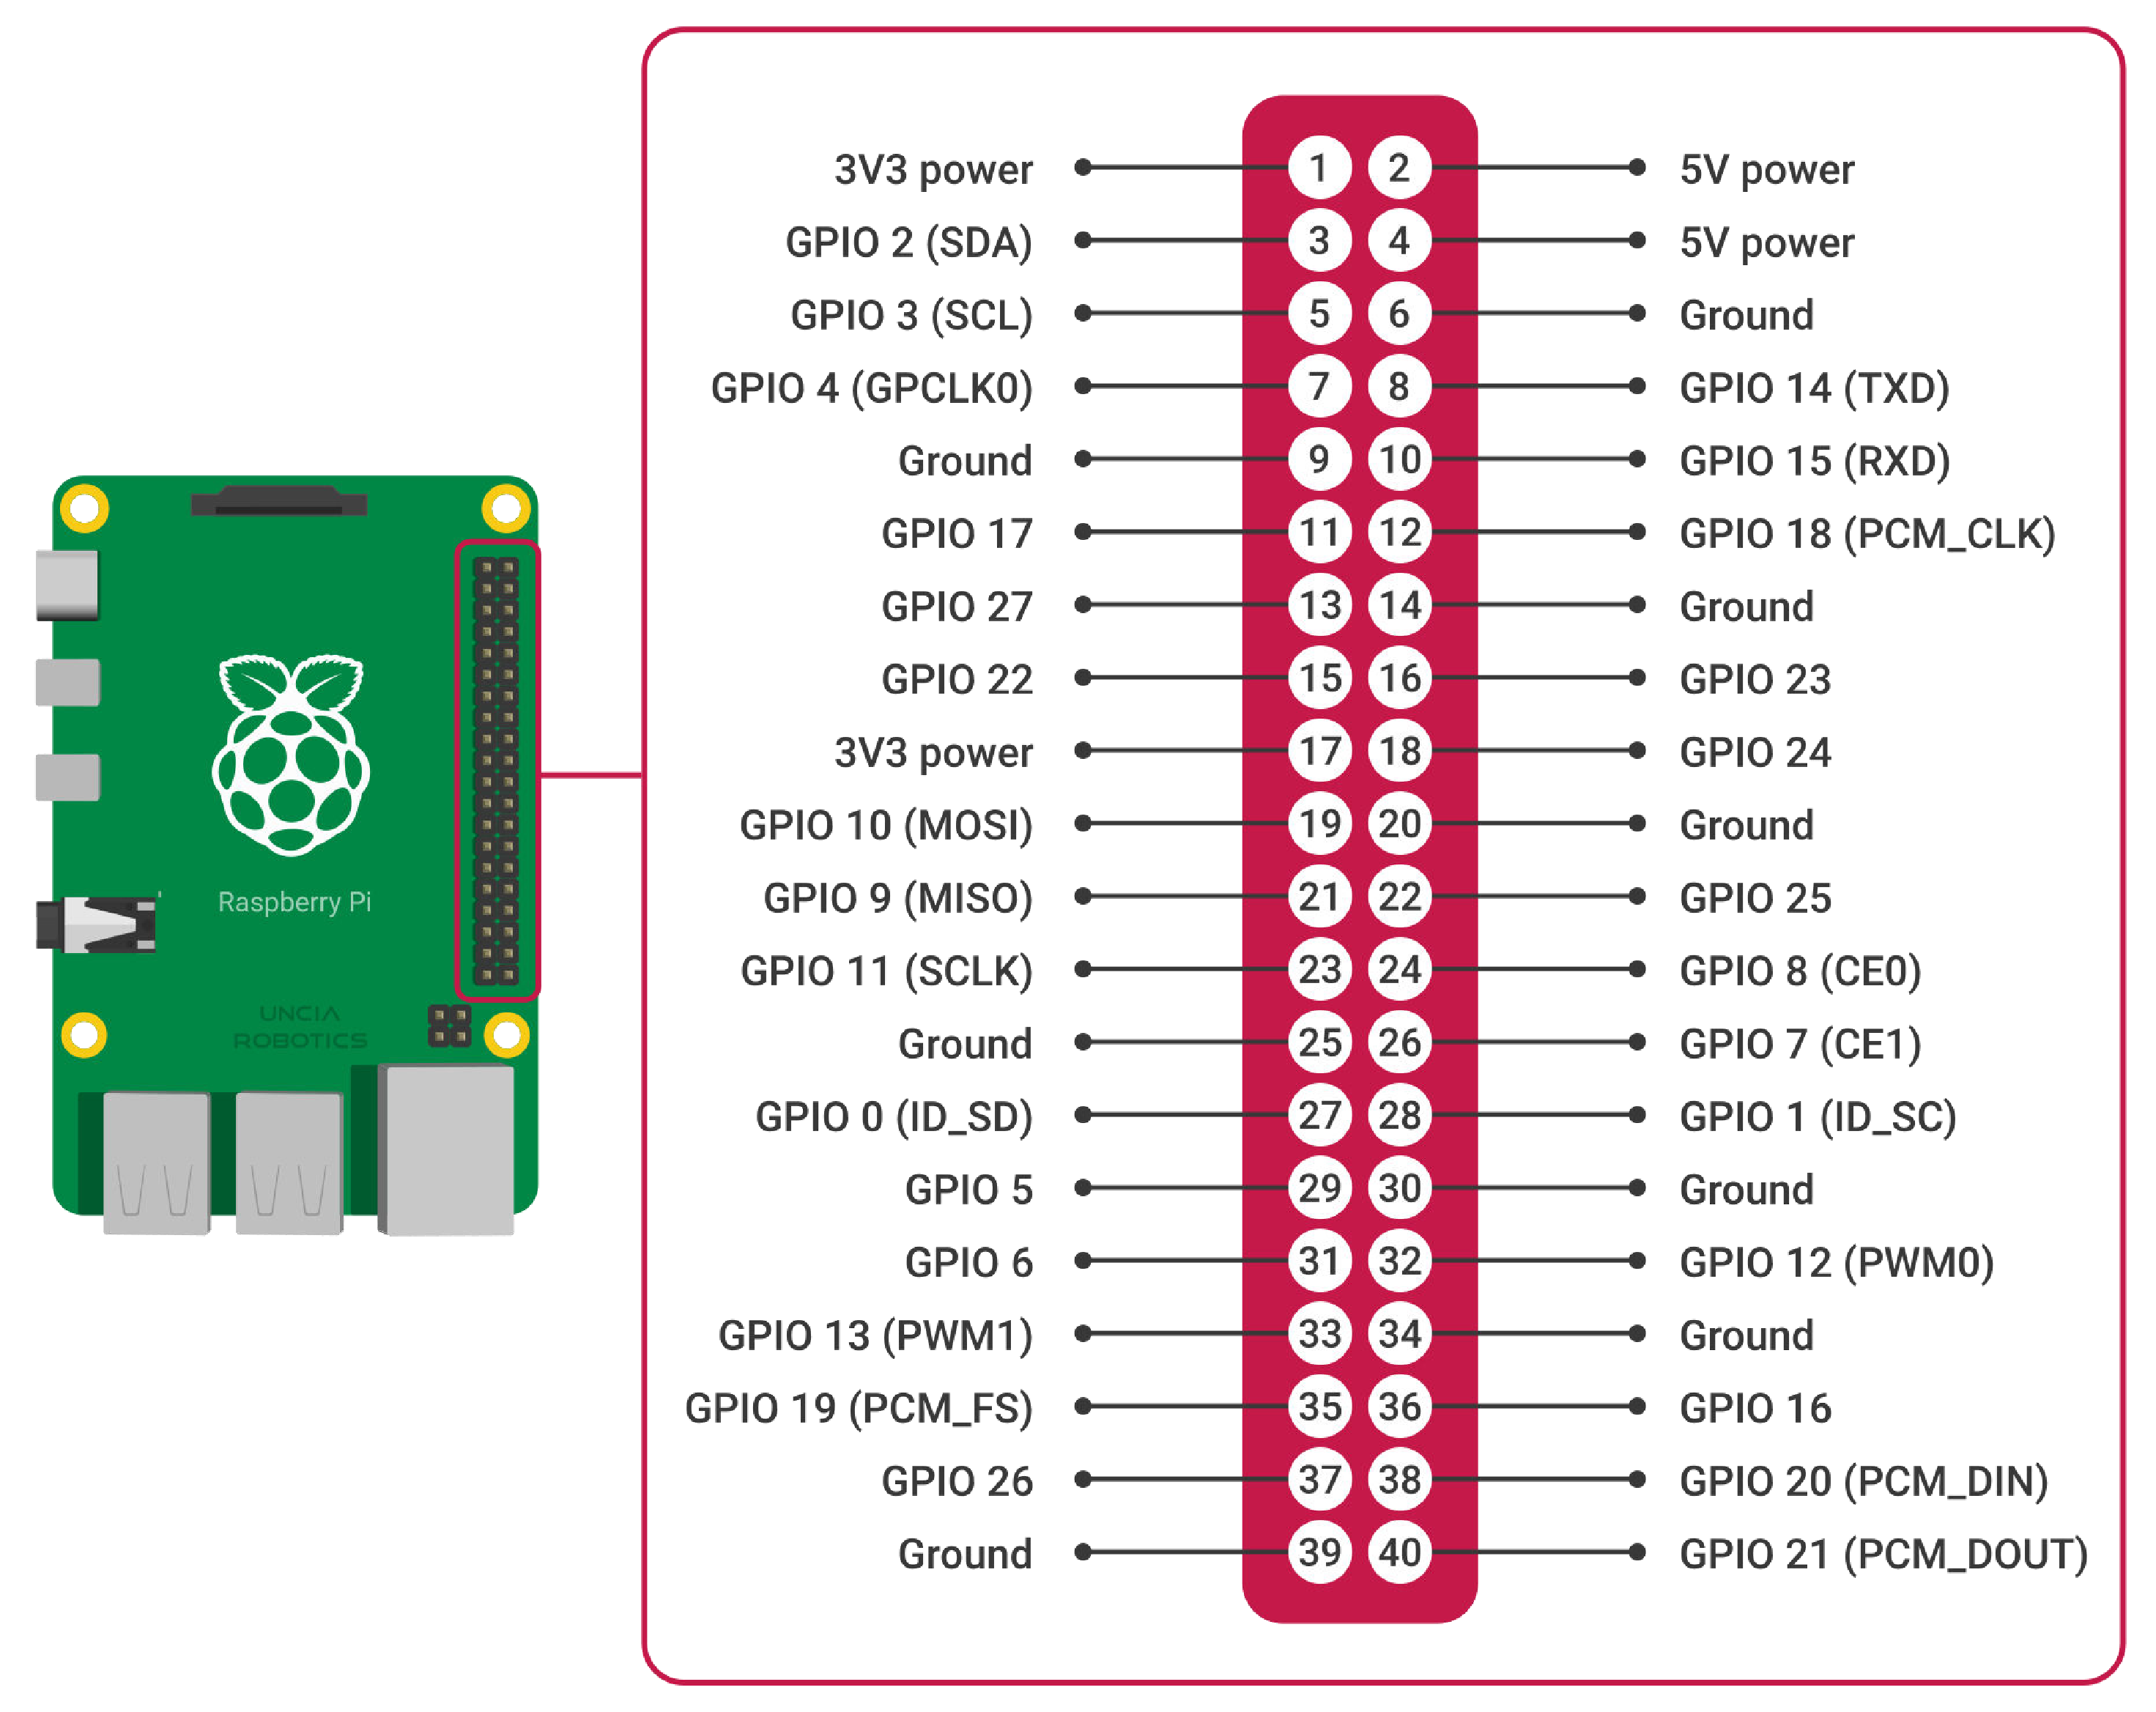
\includegraphics[width=14cm]{figures/Raspberry-Pinout.pdf}
	% \vspace{-15pt}
	\caption{Arduino针脚}
	\vspace{-15pt}
\end{figure}

\clearpage
\sectionone{接口说明和功能说明}
\begin{multicols}{2}
	\sectiontwo{I2C}
	\sectiontwo{SPI}
\end{multicols}
\end{document}